\documentclass[a4paper, twocolumn]{article}
\author{José Duarte}
\title{Concurrency \& Parallelism\\Test 1 - 2015/16}

\usepackage{listings}
\lstset{basicstyle=\ttfamily}

\usepackage{geometry}
\geometry{
    left=15mm,
    right=15mm,
    top=15mm,
    bottom=20mm,
    heightrounded
}

\usepackage{tikz}
\usepackage{hyperref}
\usepackage{amsmath}

\begin{document}
\maketitle
\section{Question 1}
\subsection{a)}
Loop iterations should not have dependencies with other loop iterations.

\subsection{b)}
Loop unrolling is an optimization technique in which a \texttt{for} loop is written as if there was no loop.
For example, the following loop:
\begin{lstlisting}
for (int i = 0; i < 4; i++) {
    print("Hello, World!");
}
\end{lstlisting}
Becomes:
\begin{lstlisting}
print("Hello, World!");
print("Hello, World!");
print("Hello, World!");
print("Hello, World!");
\end{lstlisting}

\subsection{c)}\label{q:1:c}
\begin{lstlisting}
for (int i = 0; i <n; i+=4) {
    sum += data[i];
    sum += data[i+1];
    sum += data[i+2];
    sum += data[i+3];
}
\end{lstlisting}
Or:
\begin{lstlisting}
for (int i = 0; i <n; i+=4) {
    out[0] += data[i];
    out[1] += data[i+1];
    out[2] += data[i+2];
    out[3] += data[i+3];
}
sum += out[0] + out[1] +
    out[2] + out[3];
\end{lstlisting}

\subsection{d)}
No because the overhead of instantiating a task for one simple sum would not be worth the performance.
If using the first approach from \autoref{q:1:c} the variable would also be shared which would not work as well.

\section{Question 2}
Since each GPU has double the performance of a CPU we assume that instead of 4 GPUs,
we have 8 CPUs.
We also have a fixed input size so we can use Amdahl's Law.
\begin{equation*}
    \begin{split}
        S_p & \le \frac{1}{f + \frac{1-f}{p}}\\
        S_p & \le \frac{1}{0.25 + \frac{0.75}{8}}\\
        S_p & \le 2.91\\
    \end{split}
\end{equation*}
\section{Question 3}
\subsection{a)}
When multiple processing units are required to execute a task and only one processing unit can execute it at a time.

\subsection{b)}
Cooperation occurs when processing units are required to wait for others to progress.

\subsection{c)}
Control point in which every processing unit is required to wait for the others.

\subsection{d)}
The relative size of a task/approach.

\subsection{e)}
Measurement of speedup for a fixed problem size, scaling with processing units.

\subsection{f)}
Identical operations applied to concurrently to different elements.

\subsection{g)}
Multiple tasks running in a concurrent fashion over multiple data.

\subsection{h)}
Relationship between two items in which one is required to execute before the other.

\section{Question 4}
\subsection{a)}
Read-After-Write since $S_2$ reads \texttt{x} after $S_1$ writes to it.

\subsection{b)}
Write-After-Read since $S_2$ writes to \texttt{y} after $S_1$ reads from it.

\subsection{c)}
N/A since it both writes are in different statements and the values are not read.

\subsection{d)}
Write-After-Write since $S_2$ writes to \texttt{x} after $S_1$ writes to it.

\section{Question 5}
\begin{figure}[h]
    \centering
    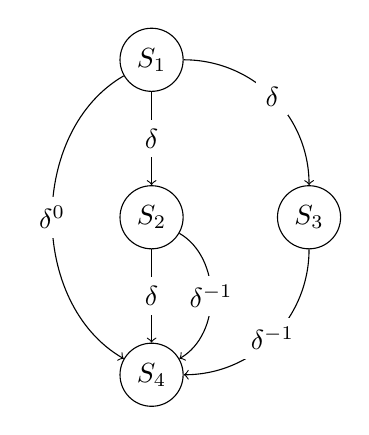
\begin{tikzpicture}[node distance=2cm]
        \node[circle, draw] (s1) {$S_1$};
        \node[circle, draw, below of=s1] (s2) {$S_2$};
        \node[circle, draw, right of=s2] (s3) {$S_3$};
        \node[circle, draw, below of=s2] (s4) {$S_4$};
        \draw[->] (s1) -- node[fill=white] {$\delta$} (s2);
        \draw[->] (s1) to[out=0, in=90] node[fill=white] {$\delta$} (s3);
        \draw[->] (s2) -- node[fill=white] {$\delta$} (s4);
        \draw[->] (s2) to[out=-30, in=30] node[fill=white] {$\delta^{-1}$} (s4);
        \draw[->] (s3) to[out=-90, in=0] node[fill=white] {$\delta^{-1}$} (s4);
        \draw[->] (s1) to[out=-150, in=150] node[fill=white] {$\delta^{0}$} (s4);
    \end{tikzpicture}
    \label{}
\end{figure}

\section{Question 6}

\section{Question 7}
Cilk+ is easier to program and requires less effort from the programmer.
Pthreads give fine-grain control.

\section{Question 8}
\begin{itemize}
    \item SISD - Serial Processors
    \item SIMD - Modern CPU's
    \item MISD - None
    \item MIMD - Distributed Cluster
\end{itemize}

\section{Question 9}
Both can lead to data consistency problems,
crossbar switching has an high incremental cost and accesses to memory are not equidistant,
the lack of a shared link improves bandwidth (comparing to bus based which shares the links).

\section{Question 10}
The map function applies one function over a collection of elements, returning the resulting collection.
The reduce function uses one function to reduce a collection of elements to a single element.

\section{Question 11}
Consider document $d$ as a set of words ${w_1, w_2, \dots, w_m}$ of size $m$,
$D$ is then the set of documents ${d_1, d_2, \dots, d_n}$.
Each document $d$ has an associated unique ID, for simplicity we consider the ID to be the number of the document $1, 2, \dots, n$.
At the document level we map $d$ to tuples of $(id, w_m, 1)$ and
then reduce to a collection of unique tuples
(in the sense that no two tuples from the same document share the same keyword),
this allows for relevance ranking.
At a global level we reduce all resulting collections $D'$ to a single collection containing tuples of $(w, {d_1, d_2, \dots, d_n})$
(that is, the word and the documents that contain it).
\end{document}